\section{The GoT Distributed Computing Model}
\label{sec:spacetime}
% Introduction
As mentioned before, the underlying distributed computing model has a dominant influence on the feasibility of an interactive debugger. Our interactive debugger, GoTcha, is designed for a specific distributed programming model called Global Object Tracker (GoT)~\cite{got}. Specifically, GoTcha is built as a debugger for a Python implementation of GoT called Spacetime. In this section, we describe GoT, and explain its design features that are relevant to GoTcha. 

\subsection{GoT: Git, but for Objects}
A Spacetime application consists of many nodes, called GoT nodes, that perform tasks asynchronously within the distributed application. The GoT nodes share among themselves a collection of objects. Each of these nodes can be executed in different machines, communicating the changes to the state of the shared objects via the network. What is unique about GoT is that the synchronization of object state among the distributed nodes is seen as a version control problem, with a solution that is modeled after Git~\cite{got}. 

All GoT nodes that are part of the same spacetime application have a repository of the shared objects, called a dataframe. The dataframe is akin to a Git repository, and, like a Git repository, it has two components: a snapshot and a version history, as shown in Figure~\ref{fig:gotnode}. The snapshot, analogous to the staging area in Git, defines the local state of the node. All changes made by the application code on the local dataframe are first staged in this snapshot. The version history, on the other hand, is the published state of the node. Like in Git, changes can be moved from the staging area to the version history using the {\em commit} primitive, and the snapshot can be made up to date with the latest version in the version history by using the {\em checkout} primitive. Inter-node communication happens using {\em push} and {\em fetch} requests, used to communicate updates in version histories between nodes. 

When the version history at a node receives changes (via {\em commit}, {\em push} or {\em fetch}), a conflict with concurrent local changes is possible and must be resolved.  While in Git conflicts are resolved manually by the user, and only on a {\em fetch}, in GoT, conflicts are resolved automatically, at the node receiving the changes, and irrespective of the primitive used. Automatic conflict resolution is achieved via programmer-defined three-way merge functions that are invoked when conflicts are detected.

% In Git, a conflict detected on a push is rejected; conflicts can only be resolved, by the user, at a repository fetching changes. In GoT, conflicts are resolved on both push and fetch requests, and the node receiving the changes is responsible for the resolution. Like Git, conflicts are resolved using three-way merge functions.

The APIs supported by the dataframe are shown Table~\ref{tbl:api}; this table can be used as a quick reference for the API calls in the example explained next.

\begin{table*}
  \begin{tabular}{lll}
    \toprule
    Dataframe API & Equivalent Git API & Purpose \\
    \midrule
    read\_\{one, all\} & N/A & Read objects from local snapshot. \\
    add\_\{one, many\} & git add <untracked> & Add new objects to local snapshot. \\
    delete\_\{one, all\} & git rm <files> & Delete objects from local snapshot. \\
    \midrule
     & git add <modified> & Objects are locally modified which is tracked by the local snapshot. \\
    \midrule
    commit & git commit & Write staged changes in local snapshot to local version history. \\
    checkout & git checkout & Update local snapshot to the local version history HEAD. \\
    \midrule
    push & git push & Write changes in local version history to a remote version history. \\
    fetch & git fetch \&\& git merge & Get changes from remote version history to local version history. \\
    pull & git pull & fetch and then checkout. \\
    \bottomrule
  \end{tabular}
  \caption{API table for a dataframe}
  \label{tbl:api}
\end{table*}

\subsection{GoT Example: Distributed Word Frequency Counter}
% The running example
The example that we use is a distributed word frequency counter. The application takes a file as input and shards it by line. These lines are distributed to several remotely located workers which tokenize and count the frequency of the tokens in the lines. The partial counts are then aggregated and presented by the application as the final word frequency tally. 

% Nodes in the example.
The distributed word frequency counter application has two types of GoT nodes: WordCounter and Grouper. The Grouper node controls the execution of this Spacetime application. It is responsible for sharding the input files into lines and aggregating partial word frequency counts to reach the final tally. The WordCounter node is responsible for tokenizing and counting the word frequencies in each line. 

\begin{figure}
\centering
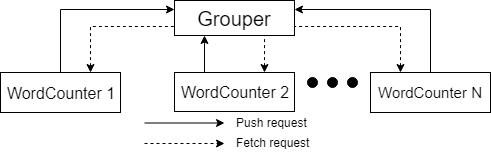
\includegraphics[width=0.45\textwidth]{images/network.png}
\caption{Network topology of an example distributed word counting application built on Spacetime.}
\label{fig:network}
\end{figure}

% Communication in example.
WordCounter nodes are responsible for the communication in this Spacetime application. Every WordCounter node must {\em fetch} changes from, and {\em push} changes to the Grouper node. This relation between these nodes is shown in Figure~\ref{fig:network} and defines the network topology of our example application. 

\begin{figure*}
\centering
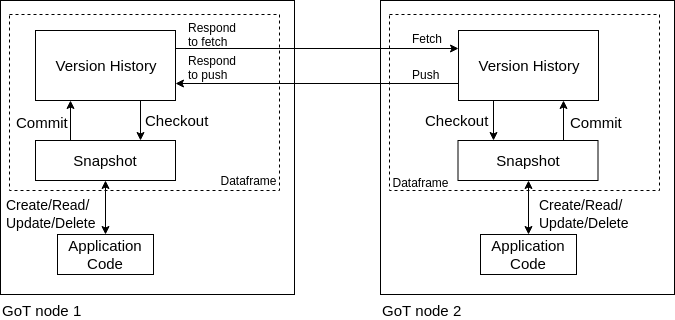
\includegraphics[width=0.66\textwidth]{images/GotNode.png}
\caption{Structure of a GoT node. Arrows denote the direction of data flow.}
\label{fig:gotnode}
\end{figure*}

% Types synched in dataframe.
The dataframes at each WordCounter and Grouper nodes share objects of type Line, WordCount, and Stop that are shown in Listing~\ref{lst:datamodel}. 

\begin{lstlisting}[language=Python,basicstyle=\small, numbers=left,
label=lst:datamodel, captionpos=b, caption=The types used by the Word Counting application.]
class Line(object):
    line_num = primarykey(int)
    line = dimension(str)
    def __init__(self,line_num,line):
        self.line_num = line_num
        self.line = line
    def process(self):
        # a simple tokenizer
        return self.line.strip().split()
        
class WordCount(object):
    word = primarykey(str)
    count = dimension(int)
    def __init__(self,word,count):
        self.word = word
        self.count = count

class Stop(object):
    index = primarykey(int)
    accepted = dimension(bool)
    def __init__(self, index):
        self.index = index
        self.accepted = False

\end{lstlisting}

% Declaration of Spacetime types
All types registered to the dataframe have list of attributes marked as dimensions of the type, that declare the attributes to be stored and tracked in the dataframe. One dimension in each type is a special attribute and is defined as the primarykey. Objects are stored and retrieved by Spacetime by the value of this primarykey attribute. 

% Types used in the example.
Objects of type Line are shards of the input file. The dimension line\_num (defined in line 2) is the primary key, of type integer, that represents the line number in the input file. The dimension, line (line 3), stores the contents of the line as a string. Objects of type WordCount store the word frequency for a unique token and have two dimensions: the primarkey, word (line 12), is a string representing the token, and count (line 13), is an integer representing the frequency of that token. WordCounter Nodes communicate completion using objects of type Stop having two dimensions: the, primarykey, index (line 19), an unique identifier representing a single WordCounter worker, and accepted (line 20), which is set to True by the WordCounter node signalling the completion of its task. Any state in attributes outside these dimensions is purely a local state, and is not tracked and shared by the dataframe.

\vspace{3cm}

\begin{lstlisting}[language=Python,basicstyle=\small, numbers=left, 
label=lst:grouper, captionpos=b, caption=The Grouper node.]
def Grouper(df,filename,num_count):
    i = 0
    for line in open(filename):
        df.add_one(Line, Line(i,line))
        df.commit(); i += 1;
    df.add_many(Stop,
      [Stop(n) for n in range(num_count)])
    df.commit()
    while not all(
          s.accepted
          for s in df.read_all(Stop)):
        df.checkout()
    for w in df.read_all(WordCount):
        print(w.word, w.count)
        
if __name__ == "__main__":
    filename, num_count = sys.argv[1:]
    grouper_node = Node(
        Grouper, server_port=8000
        Types=[Line,WordCount,Stop])
    grouper_node.start(filename,num_count)
\end{lstlisting}

% Describing grouper node initialization
Listing~\ref{lst:grouper} shows part of the application code for an instance of the Grouper node. The grouper\_node is instantiated (lines 18-20) with the application code, defined by the function Grouper, along with the types to be stored in the dataframe, and the port on which to listen to incoming connections. The grouper\_node is launched using the blocking call, start (line 21), and takes in the parameters that must be passed to this instance of the Grouper node: the input file and the number of WordCounter nodes that are going to be launched. 

% Describing grouper node execution
The Grouper function  (line 1) that is executed receives the repository, dataframe, as the first parameter, and all run-time supplied parameters as the additional parameters. The node iterates over each line in the input file, creating new Line objects for each line. The Line objects are added to the local dataframe (line 4), similar to how new files are added to a changelist in git. After each Line object is added, these staged changes are committed to the dataframe (line 5) and are available to any remote dataframe that pulls from it. After all Line objects are added, Stop objects are added, one for each WordCounter worker in the application, and committed to the dataframe (line 6-7). Grouper now has to wait for all WordCounter workers to finish tokenizing the lines that it has published, and the state of the Stop object acts as that signal (Lines 9-12). Once every worker has accepted the Stop object associated with it, the Grouper reads all the WordCount objects in the repository and displays the word frequency to the user.

\begin{lstlisting}[language=Python,basicstyle=\small, numbers=left, 
label=lst:word_counter, captionpos=b, caption=The Word Counter node.]
def WordCounter(df,index,num_count):
    line_num=index; stop=None; line=None
    while not stop or line:
        df.pull()
        line = df.read_one(Line,line_num)
        if line:
            for word in line.process():
                # reads from the snapshot
                word_obj = df.read_one(
                    WordCount,word)
                if not word_obj:
                    word_obj = WordCount(
                        word,0)
                    df.add_one(word_obj)
                # changes only snapshot
                word_obj.count += 1
            line_num += num_count
        stop = df.read_one(Stop,index)
        # commit changes 
        # to version history
        # and push these changes
        # to remote node.
        df.commit(); df.push()
    stop.accepted = True
    df.commit()
    df.push()
if __name__ == "__main__":
    workers = []
    address = sys.argv[1]
    num_workers = int(sys.argv[2])
    for i in range(num_workers):
        wnode = Node(
            WordCounter,
            Types=[Line,WordCount,Stop],
            remote=(address, 8000))
        wnode.start_async(i, num_workers)
        workers.append(wnode)
    for w in workers:
        w.join()
\end{lstlisting}

% How to launch word counter
Listing~\ref{lst:word_counter} shows part of the code for an instance of the WordCounter. Multiple instances of the WordCounter node are instantiated with the remote address of the Grouper node, and the same Types that Grouper uses (lines 32-35). Each instance is started asynchronously with the parameters that it needs (line 36). 

% What word counter does.
The application code for WordCounter (function WordCounter shown in lines 1-26) also takes the dataframe as the first parameter. An independent and new dataframe is created for each instance of WordCounter, and they all have the same Grouper node as the remote node. The WordCounter keeps pulling changes from the remote node (line 4) for as long as there is a new line to read in the updated local dataframe and until a Stop object associated with the instance is read in the local dataframe. In each pull cycle, the WordCounter reads a Line object from the local dataframe, using index (line 5), and tokenizes it (line 7). For every word in the token list, the node retrieves the WordCount object associated with the word from the dataframe (line 9), creating and new object if it does not exist (line 11-14), and increments the count dimension in the object by one (line 16). These updates (both new objects, and updates to existing objects), staged in the local snapshot, are committed to the local dataframe and pushed to the remote Grouper node (line 23). The WordCounter ends operations if after pulling updates from Grouper, a Stop object is present in the dataframe, and there are no new Line objects to read. The stop object is accepted by setting the accepted dimension to True and this update is committed and pushed to Grouper as the last operations by the WordCounter node.

\subsection{Dataframe: Object Repository}
% What is the dataframe
To the code in each of the GoT nodes, the dataframe acts an object heap that consists of in-memory objects that are under version control. As explained above, the dataframe in each node has two components: a snapshot and an version history.

% What does the data structure of the history look like? 
The version history is stored as a directed acyclic graph where each vertex of the graph represents one version of the state and has a globally unique identifier that labels it and each directed edge of the graph represents a causal ``happened-after'' relation. Each edge is associated with a delta of state changes (diff) that when applied to the state of the objects at the source version transform it to the state of the objects at the destination version. The latest version of the node state (called the HEAD) is the state of the node that is observable to the other nodes in the application. Changes that are staged in the snapshot cannot be observed by external nodes until they are put into the version history. 

% memory management.
An edge with an associated delta is added into the graph for each new version of the state and, therefore, memory usage of the application can potentially be high. To manage the memory, Spacetime implements an effective garbage collector in each node that cleans up obsolete versions.

% Commit and Checkout
Changes that are made to the objects in the application code, are staged in the snapshot. When the {\em commit} primitive is invoked, a new version is created in the version history, representing the newly committed state. An edge is added from the last version the snapshot was in, to the newly created version in the version history. The diff that was committed is then associated with this edge. Changes to the version history, updated by external nodes, are introduced to the snapshot via the {\em checkout} primitive.

% fetch and push.
Inter-node communication only happens between the version histories of the corresponding nodes. As seen in the example and like Git, nodes communicate changes between version histories using the {\em fetch} and {\em push} primitives present in the dataframe. {\em Fetch} retrieves changes published to the version history in a remote GoT node and applies the changes to the local version history. {\em Push} takes changes published to the local version history and delivers it to a remote GoT node. GoT takes advantage of the diffs stored in the version histories to communicate via delta encoding, reducing the amount of data transferred between nodes. 

\subsection{Conflict Detection and Resolution}
% Generic conflict detection and resolution
Conflicts are detected (at any node that is receiving data), when an update received is a change from a version that is not the HEAD version in the local version history. Intuitively, this means that at least two different nodes committed concurrent changes after having read the exact same version. When conflicts are detected, they are resolved using a user defined three way merge function that includes the state that was read (the original), the changes already in the version history (yours) and the conflicting changes that are incoming (theirs). The output of the merge function, much like the merge resolution in git, adds a new merged version to the version history that has a happened-after relation with both the diverging versions. 

% Specific to example conflict resolution
In the WordCounter example, the state of the WordCount objects created and updated by different WordCounter nodes can be in conflict with each other when changes are pushed to the Grouper node. For example, if two WordCounter nodes concurrently read the same word in two different lines and the word has not been observed before, both the nodes would create a new WordCount object for the word. When both changes are pushed to the Grouper node, a conflict is detected and a merge function is called.

\begin{lstlisting}[language=Python,basicstyle=\small, numbers=left, 
label=lst:merge, captionpos=b, caption=Merge function used at the Grouper node.]
def merge(conf_iter,orig_df,
          your_df,their_df):
    your_df.update_not_conflicting(
        their_df)
    for orig,yours,theirs in conf_iter:
        assert isinstance(yours,WordCounter)
        yours.count += theirs.count
    return your_df
...
    # Updated Node initialization
    grouper_node = Node(
        Grouper,server_port=8000,
        Types=[Line,WordCount,Stop],
        conflict_resolver=merge)
\end{lstlisting}

        % if original:
        %   yours.count += theirs.count - original.count

% Structure of the merge function
An example merge function is shown in Listing~\ref{lst:merge}. This function is called asynchronously when a conflict is detected, and is used to only to reconcile conflicting state updates. The merge function receives four parameters: an iterator of all objects that have direct contradictory changes that cannot be auto resolved ({\em conf\_iter}), as well as three snapshots of the state, one for the point where the computation forked ({\em orig\_df}), and two for the version at end of the conflicting paths ({\em your\_df}, {\em their\_df}). 

% How does the merge example work
In the merge function shown, objects (Line, WordCount, and Stop objects) that are new or modified in the incoming change but do not have conflicting changes in the local history are first accepted (line 3). For the objects that are in conflict (only WordCount objects can be in conflict), we read the states at three versions of the objects: the state at the fork version, and the two states at the conflicting versions -- {\em orig}, {\em yours}, and {\em theirs} from the iterator (line 3), respectively. Then, the dimension count in objects that have been updated together are added up and stored in the object tracked by the {\em your\_df} snapshot. At the end, this modified version of {\em your\_df} is considered to be the reconciled state and returned to the version history. 

% There is a bug, and we'll correct it later.
There is a bug in this merge function as it does not add counts correctly. We will use this bug to demonstrate the capabilities of the interactive debugger. For quick reference, the correct merge function is shown in Listing~\ref{lst:correct_merge} at the end of Section~\ref{sec:debug_arch}.
